\section{Price and license}
\label{sec:prices}

Table~\ref{tab:prices} quotes each vendor's own price page as read on 2026-09-25 (\code{docs/price\_survey\_2026-09-25.txt}). The products fall into three groups: desktop tools under an open license with no charge; desktop tools with a free non-commercial tier and a metered or per-seat commercial tier; and cloud services billed by the hour of session or training time, on top of which the vendor's compute and storage are billed separately.

\begin{table}[htbp]
\caption{Stated prices, verbatim from the vendor page named in the price survey. ``No list price'' means the page carries none.}
\label{tab:prices}
\small
\begin{tabular}{@{}L{3.4cm}L{2.0cm}L{9.8cm}@{}}
\toprule
Product & Form & Price as stated \\
\midrule
DiGiTerra 0.1.0 & desktop or hosted & MIT license, no charge \\
Orange 3 & desktop & GNU General Public License \\
KNIME Analytics Platform & desktop & ``Free''; KNIME Pro ``Starts at \$19 / month''; Team ``Starts at \$99 / month'' for 3 members, ``\$49/month'' each further member; Business Hub ``Pricing available on request'' \\
Altair AI Studio & desktop & ``available to everyone for free for non-commercial purposes'' as a ``Renewable one-year license''; commercial use metered in Altair Units, ``The baseline for using Altair AI Studio is 20 Altair Units'', no unit price on the pages read \\
H2O-3 Flow & local server & Apache 2.0; Flow ``is deprecated and will be removed in a future release'' \\
Amazon SageMaker Canvas & cloud & ``\$1.9/hour'' workspace session; ``a 2-month free tier \ldots\ up to 160 hours/month''; training ``\$2.03 - \$4.89 per hour of training time'' \\
Azure Machine Learning & cloud & ``there is no additional charge to use Azure Machine Learning''; compute, storage, key vault, registry and insights billed separately \\
Google Vertex AI AutoML tabular & cloud & Training ``\$21.252 / 1 hour''; inference ``Same price as inference for custom-trained models'' \\
Weka & desktop & GNU General Public License \\
JASP & desktop & GPLv2 and AGPLv3 \\
jamovi & desktop, cloud & Desktop free; Cloud ``Guest'' free, ``Priority'' ``Priced by region'', ``Teams'' custom quote \\
DataRobot & SaaS, self-managed & No list price; ``Try DataRobot'', ``Request a Demo'' \\
Microsoft Excel (E1 reference) & desktop & Office Home 2024 ``\$179.99''; Microsoft 365 Personal ``\$99.99/year'' or ``\$9.99/month'' \\
\bottomrule
\end{tabular}
\end{table}

\begin{figure}[htbp]
\centering
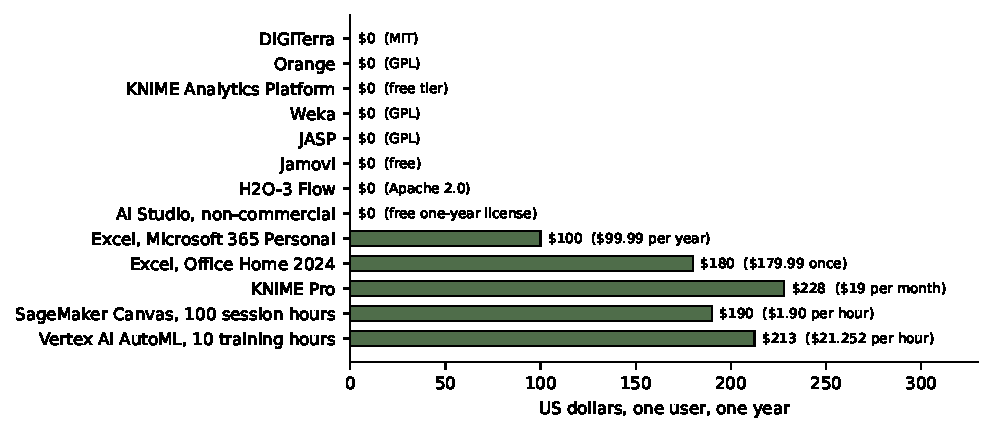
\includegraphics[width=0.85\textwidth]{fig_price_scenario}
\caption{Stated price under one scenario: one user, one year, about 100 hours of modeling. Desktop tools cost their license; SageMaker Canvas is charged at the session rate for 100 hours; Vertex AI at the training rate for 10 training hours (session time is not billed as such); KNIME Pro at twelve months. Azure Machine Learning, DataRobot and AI Studio's commercial tier carry no list price on the pages read and are not drawn. Excel is shown under both purchase forms. Source: \code{docs/price\_survey\_2026-09-25.txt}.}
\label{fig:price}
\end{figure}

The scenario in Figure~\ref{fig:price} is one reading of the stated prices, not a total cost of ownership. A cloud service's bill depends on the compute chosen, the data stored and the hours logged in, and the free tiers change; a desktop tool's cost is the machine the group already owns. The point the figure carries is narrower: for the workflow the product comparison describes, a fitted and documented model on one table, every desktop product in the table is available at no charge, and the cloud products bill from the first hour after their free tier.
